\section{Implementation}
\label{sec:impl}

We implement \sys as an end-to-end pipeline in Python. Each of the four agents is realized as an LLM-backed module driven by \texttt{claude-sonnet-5} at temperature 0.7, orchestrated as a LangGraph state machine through a common controller that manages prompting, tool invocation, and the per-agent execute-and-repair loop. Agents communicate through a shared, structured project state (the current source tree, the interface delta emitted by the \emph{LSA}, and the running verification log), serialized as JSON so that any agent can inspect the artifacts produced upstream.

\textbf{Execution and sandboxing.}
Local verification has to run code that a language model has just written, so every candidate clone is executed rather than inspected. \sys copies each candidate into a fresh temporary directory and runs it there with the host Python interpreter under a wall-clock limit, so that a clone which hangs is abandoned instead of stalling the batch. Four things are captured: whether the file compiles, the process exit status, everything written to standard output and standard error, and the text of any assertion that failed. That output is handed back to the responsible agent \emph{unedited}: the agent repairs against the actual traceback rather than a summary of it. The isolation is filesystem-level and not a container: each run gets its own directory, but a clone that opened a network connection or wrote outside that directory would not be stopped. This is acceptable here because the corpus is our own and every generated file is read before it is executed; applying \sys to untrusted programs would require a container or VM boundary. We state this as a limitation of the current implementation rather than a property of the design.

\textbf{Test harness.}
The \emph{VCA} discovers and drives whatever test assets accompany a subject program (unit and integration tests as well as recorded reference input/output traces) through a uniform adapter, so that heterogeneous test formats present a single pass/fail/attribution interface to the pipeline.

\textbf{How glue is applied.}
The \emph{GSA} does not emit a rewritten file. It first analyzes each call site that touches the outgoing library and decides which of them require an adapter; it then enters an \emph{agent--computer interface} (ACI) editing session over the real file, with \texttt{open}, \texttt{search\_file}, \texttt{goto}, \texttt{scroll}, \texttt{edit} and \texttt{submit} operations. Every \texttt{edit} is checked before it is applied and is rejected outright if the replacement text would not parse, so the model receives the syntax error and retries instead of committing a broken file. Editing line ranges in the actual file, rather than regenerating the module, keeps the diff small and makes an unrelated rewrite visible.

Two invariants are enforced outside the model. The session may not edit import statements: that rewrite is performed deterministically afterwards, using the module root resolved from the file's own imports rather than from the distribution name, because the two differ: \texttt{paho-mqtt} is imported as \texttt{paho}, \texttt{simple-pid} as \texttt{simple\_pid}. After the session, each call site the analysis recorded is repointed at its wrapper by an AST transformation that matches the recorded call text exactly and passes arguments through unchanged; imports the migration has left unreferenced are then deleted, and a patch that still imports the removed library is rejected and returned to the \emph{GSA} with the offending line attached. We adopted the deterministic path after observing the editing session rewrite a call site other than the one its own analysis had identified, leaving an orphaned factory that still constructed the outgoing library.

\textbf{Equivalence oracle.}
To certify the results reported in Section~\ref{sec:results}, we score every clone with a five-layer source-level oracle, applied in increasing order of cost. This is an independent audit of the finished clone, run after the pipeline has already stopped; Section~\ref{sec:approach} describes the separate, deliberately narrower check the VCA itself runs live. The first layer validates that the clone's imports resolve and that the migrated-away distribution is genuinely absent. The second replays recorded golden vectors (inputs and expected outputs captured from the pristine original) at zero numerical tolerance. The third checks program invariants that must hold irrespective of implementation, such as monotonicity of a control output or the reachability of every declared state. The fourth runs the subject's own \texttt{pytest} suite against the clone. A verdict of equivalence requires all layers to pass, and the first to fail identifies the responsible agent directly.

The fifth layer was added mid-study, in response to a systematic blind spot the first four share. Every subject dependency-injects its I/O client so that its tests can run without live hardware, which means the factory function that actually constructs the substituted library (\texttt{\_default\_client}, \texttt{\_default\_smtp}) runs only when the caller injects nothing, and is therefore executed neither by the test suite nor by the oracle's probes. It is also exactly where the substitution lives. The fifth layer calls that factory directly against \texttt{192.0.2.1}, an address reserved for documentation (RFC~5737) that is routable-looking but guaranteed dead, and classifies what comes back. A connection refusal, timeout or DNS failure is consistent with a correct migration and no server, and is recorded but never failed. A \texttt{TypeError}, \texttt{AttributeError}, \texttt{NameError} or \texttt{ValueError}, an import of a library that is neither the declared source nor the declared target, or an operating-system error naming the address we passed as though it were a filename, cannot be caused by absent hardware: the call itself is wrong, and the layer fails it. The motivating case was a clone that passed a TCP hostname to \texttt{minimalmodbus.Instrument}, whose first parameter is a serial device path; it scored 5/5 on its suite and satisfied all four earlier layers. Across the 144 runs reported in Section~\ref{sec:results} the layer returned this verdict nine times, and was skipped on 48 runs where no factory was present or the declared library was absent from the evaluation machine.

\begin{figure}[t]
\centering
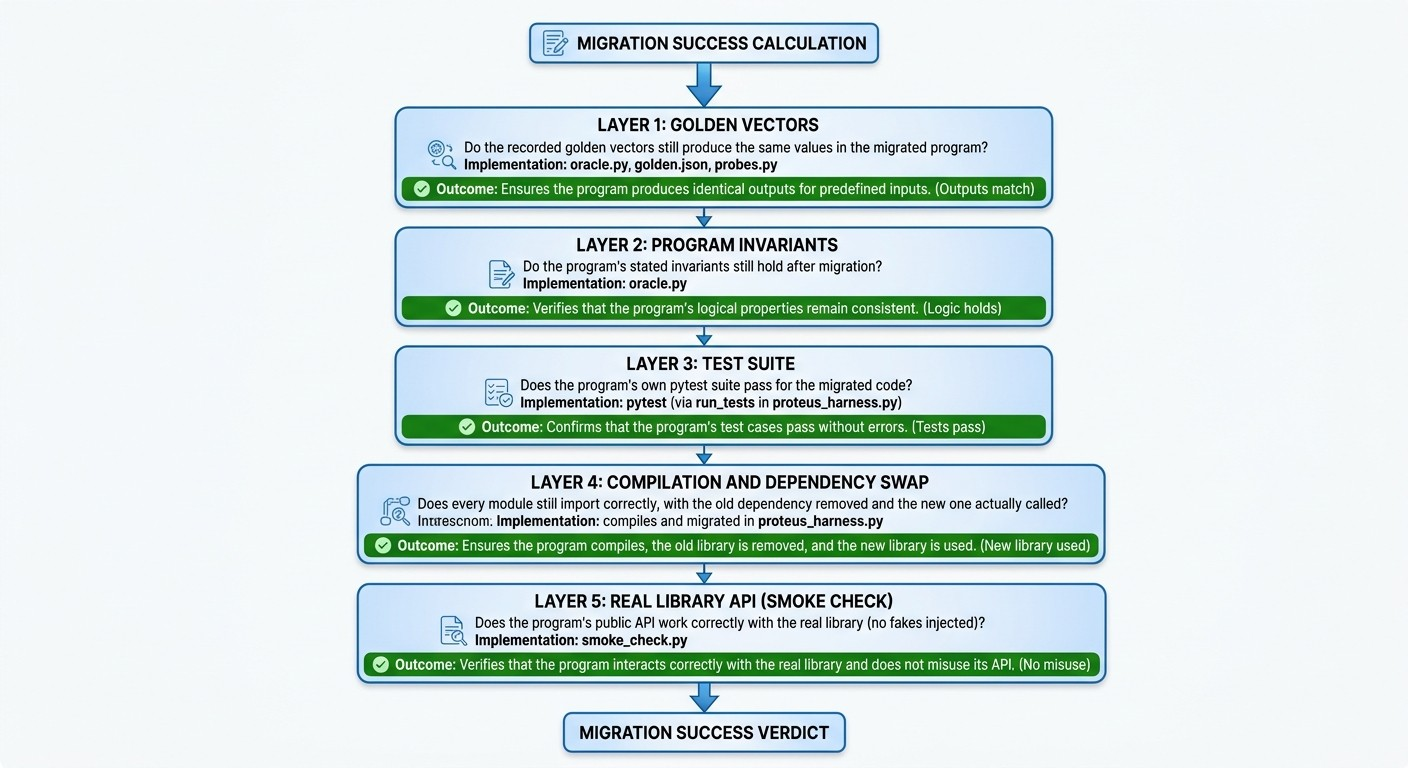
\includegraphics[width=\linewidth]{figs/migration_success_layers.jpg}
\caption{The five-layer migration-success oracle applied to every clone, in increasing order of cost. Layers 1--4 operate on paths the subject's own dependency-injected tests reach; Layer 5 is the one layer that exercises the factory function performing the substitution itself, against the real library, and is what closes the blind spot described above. A clone must pass every layer to receive a migration-success verdict, and the first layer to fail identifies the responsible agent.}
\label{fig:oracle_layers}
\end{figure}

\textbf{Scope of the global oracle.}
This scoring oracle is source-level. It is the five-layer checker described above, and every equivalence figure in Section~\ref{sec:results} comes from it. Extending confirmation to the binary level (disassembling the compiled original and clone, generating emulator execution traces, and deciding semantic equivalence from those traces, in the manner of our prior binary clone detector~\cite{agadakos2025bcd}) is a plausible next step, and would address the corpus's central weakness that dependency-injected tests never execute the migrated code path. We have not implemented it, and no result in this paper depends on it.

\paragraph{Subject Programs}
Our evaluation corpus consists of twelve Python programs from the industrial measurement and control domain, organized into four categories of increasing transformation demand and ranging in complexity from a single self-contained module to multi-file packages with internal dependencies (Section~\ref{sec:results}, Table~\ref{tab:corpus}). The programs were authored for this study rather than harvested from public repositories, a trade we revisit in Section~\ref{sec:results}: it costs external validity, and it is what makes the per-program golden vectors and invariants the oracle consumes available at all. Every subject ships a \texttt{pytest} suite and recorded input/output traces, which serve both as the \emph{VCA}'s test corpus and as ground truth for the equivalence oracle.
